\documentclass[a4paper,8pt,french,fleqn]{article}
%Packages:

%Langages:
\usepackage[french]{babel}
\usepackage{lmodern}
\usepackage[T1]{fontenc}
\usepackage[utf8]{inputenc}

%AMS maths
\usepackage{amsmath, amssymb, amsfonts}

%Mise en page
\usepackage[top=2cm, right=2cm, bottom=2cm, left=2cm]{geometry}
\usepackage{fancyhdr}
\usepackage{enumerate}
\usepackage{color}
%Définition des macros
\usepackage{amsthm}

%Figures
\usepackage{tikz}
\usepackage{graphicx}
\usepackage{wrapfig}

%Symboles mathématiques
\usepackage{latexsym}
\usepackage{bm}

%Titre et auteurs

\title{\textbf{ Projet scrabble }\\\textit{Rapport du travail fourni}}
\author{PHILIPPI Alexande \& JEANJEAN Vincent \& HBAIEB Ahmed}
\date{\today}

\begin{document}

\begin{figure}[h]
  \begin{center}
    
\includegraphics[scale=1.5]{enseirb.jpg}
    \vspace{2cm}
    \maketitle    
  \end{center}
\end{figure}

\newpage

\tableofcontents

\newpage

\section{Introduction}

Le but de ce projet était de réaliser une intelligence artificielle jouant au scrabble et sortant le meilleur coup possible à chaque tour. La complexité de ce sujet résidait notamment dans la gestion de tous les cas possibles pour poser un mot tiré du dictionnaire du scrabble. Il fallait aussi mettre en place plusieurs options : \\

\begin{itemize}

\item Une option '-m' permettant au joueur d'entrer à chaque tour de jeu les lettres dans sa main en prenant en compte les lettres disponibles. Ce mode devait aussi permettre au joueur de choisir parmis une liste de mots possibles (les 'n' meilleurs) celui qu'il voulait poser ; \\

\item Une option de sauvegarde pour pouvoir sauvegarder les lettres dans la main du joueur à chaque tour de jeu, ainsi que le nombre de points réalisés pour pouvoir ultérieurement rejouer la partie et comparer les résultats obtenus ; \\

\item Une option de sauvegarde de la grille actuelle pour pouvoir effectuer du débuggage. \\

\end{itemize}

\begin{figure}[h]
  \begin{center}
    \vspace{0.5cm}
    \includegraphics[scale=0.6]{eliot.png}
    \hspace{1.5cm}
    \includegraphics[scale=0.68]{scrabble.png}
    \caption{Grille de jeu d'Eliot à gauche et de notre programme à droite}
  \end{center}
\end{figure}

\newpage
 
\section{Démarche}

Dans un premier temps, nous avons réalisé un algorithme faisant la liste de tous les mots réalisables en fonction de la main du joueur et des mots du dictionnaire. \\

Puis nous avons cherché à placer le meilleur mot parmis tous les mots possibles au premier tour de jeu en respectant la régle du premier tour (le mot doit forcément passer par le centre de la grille). \\

Nous avons ensuite pris en compte un premier cas pour les tours de jeu suivant : le cas des mots croisés simple. Le mot placé ne devait couper qu'un unique mot ou sinon compléter un mot déjà posé :

\begin{figure}[h]
  \begin{center}
    \vspace{0.2cm}
    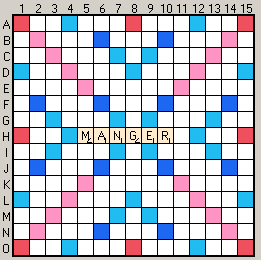
\includegraphics[scale=0.5]{cas1a.png}
    \hspace{1.5cm}
    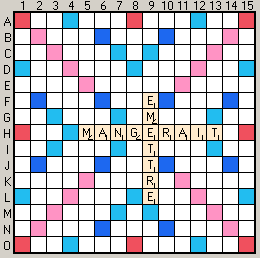
\includegraphics[scale=0.5]{cas1b.png}
  \end{center}
\end{figure}

Ensuite nous avons pris en compte le croisement de plusieurs mots déjà posés sur le plateau ainsi que le raccord de deux mots espacés mais placés sur la même ligne (mots horizontaux) ou même colonne (mots verticaux) :

\begin{figure}[h]
  \begin{center}
    \vspace{0.2cm}
    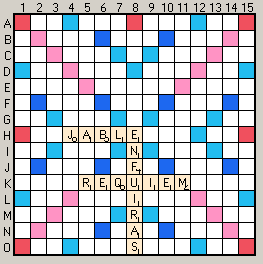
\includegraphics[scale=0.5]{cas2a.png}
    \hspace{1.5cm}
    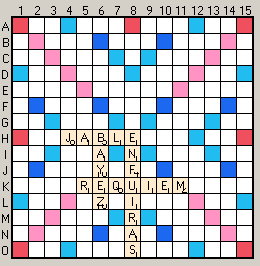
\includegraphics[scale=0.5]{cas2b.png}
  \end{center}
\end{figure}

Puis nous avons pris en compte le placement de mots superposés à d'autres mots. Cas difficile à gérer, car il fallait prendre en compte tous les mots créés, s'assurer qu'ils existaient tous, et si tel était le cas, ajouter leurs points au gain du mot : 

\begin{figure}[h]
  \begin{center}
    \vspace{0.2cm}
    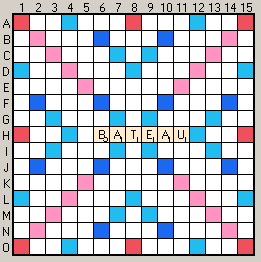
\includegraphics[scale=0.5]{cas3a.png}
    \hspace{1.5cm}
    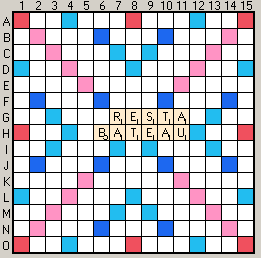
\includegraphics[scale=0.5]{cas3b.png}
  \end{center}
\end{figure}

Finalement le dernier cas à gérer correspondait à celui des mots par exemple horizontaux complétés par un mot vertical. Il est nécessaire de savoir que notre algorithme ne pouvait initialement placer que des mots qui étaient rattachés à d'autres mots du plateau, c'est pourquoi ce cas n'était pas géré s'il n'y avait pas de mots sur la ligne orthogonal au mot complété :

\begin{figure}[h]
  \begin{center}
    \vspace{0.2cm}
    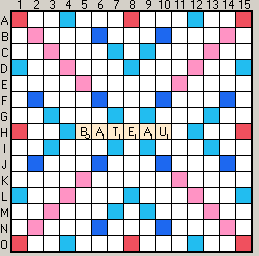
\includegraphics[scale=0.5]{cas4a.png}
    \hspace{1.5cm}
    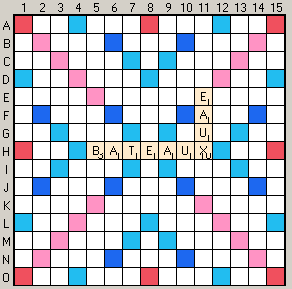
\includegraphics[scale=0.45]{cas4b.png}
  \end{center}
\end{figure}

Une fois tous ces cas gérés nous avons utilisé le temps restant pour faire des essais, notamment en comparant les résultats obtenus avec ceux obtenus par le programme Eliot. Nous en avons aussi profité pour paufiner le programme, ajouter des options comme le mode d'ajout manuel de lettres et la possibilité au joueur de choisir un mot parmis une liste de meilleurs mots possibles :

\begin{figure}[h]
  \begin{center}
    \vspace{0.2cm}
    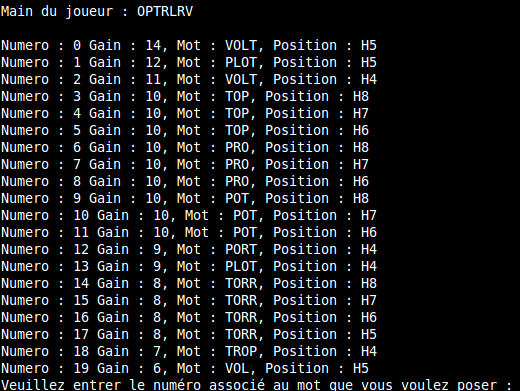
\includegraphics[scale=0.5]{choix.png}
  \end{center}
\end{figure}

\newpage

\section{Autour des algorithmes}

\subsection{Solution employée}

La méthode qui nous est venue à l'esprit en premier est la méthode 'brute force', qui consiste à étudier tous les cas possibles pour ne garder au final que la meilleure solution. A chaque tour de jeu, toutes les possibilités d'actions sont étudiées, et pour chaque cas on compare les points rapportés avec la dernière meilleure combinaison trouvée. Une fois tous les cas balayées, la meilleure combinaison trouvée est placée sur le plateau de jeu. \\ 

\subsubsection{Génération du plateau de jeu}

Pour simuler le plateau de jeu, nous avons créé une matrice de taille $15 \times 15$ initialement remplie de points, contenant des informations sur le type de case (mot compte double/triple, lettre compte double/triple) et sa disponibilité (case déjà occupée par une lettre perd ses bonus). 

\subsubsection{Tirage}

A chaque début de tour, la main du joueur est completée à 7 en respectant les probabilités d'acquisition de chaque lettres. Pour cela nous avons mis en place un tableau de 102 caractères représentant le sac que nous avons rempli manuellement en respectant les proportions de présence de chaque lettres. 

\subsubsection{Recherche du meilleur mot}

Pour trouver le meilleur mot, nous avons donc utilisé la méthode 'brute force'. Le plateau de jeu est entièrement balayé et tous les cas envisageables sont étudiées en fonctions des lettres disponibles dans la main du joueur et des mots sur le plateau. Voici le détail de la procédure de recherche du meilleur mot : \\

\begin{itemize}

\item Le programme réalise dans un premier temps un balage horizontal de la grille puis dans un second temps un balayage vertical ; \\

\item Tous les mots d'une ligne sont récupérés et enregistrés. Puis le programme étudie d'abord le premier mot, il cherche dans le dictionnaire tous les mots possibles pouvant être construits avec en fonction de la place disponible sur la ligne et des lettres dans la main du joueur ; \\

\item  Ensuite il vérifie si des mots sont déjà posés sur les lignes juste au dessus ou juste en dessous, si tel est le cas, il vérifie que tous les mots créaient orthogonalement au mot existent ; \\

\item Si jamais le mot posé fait seulement un caractére de plus que le mot du plateau, le programme va vérifier si un mot ne peut pas être posé orthogonalement pour rapporter plus de points. \\

\end{itemize}

\subsubsection{Calcul des points}

Pour chaque mot réalisable on calcule le gain apporté et on le compare avec le gain du dernier meilleur mot trouvé. Si son gain est supérieur au gain du meilleur mot trouvé alors il prend sa place.

\subsubsection{Placement du meilleur mot}

Une fois que toutes les possibilités ont été balayées, on place le dernier meilleur mot trouvé sur la grille. Les lettres du mot posé sont retirées de la main du joueur et on passe au tour de jeu suivant. Si jamais aucun mot ne peut être fait avec la main actuelle, toutes les lettres du joueur sont jetées dans le sac et le tour se termine. 

\subsubsection{Arrêt du jeu}

L'algorithme se termine lorsqu'il n'y a plus de lettre disponible dans le sac ou bien lorsque le joueur n'a pas pu jouer 10 tours de suite.

\subsubsection{Options supplémentaires}

Si l'utilisateur passe '-m' en argument du programme scrabble, il aura alors la possibilité à chaque tour de jeu de compléter manuellement sa main en respectant bien sur la disponibilité de chaque lettres. S'il passe '-n' en argument, il pourra choisir parmis 20 meilleures solutions celle qu'il veut jouer, les 20 meilleures solutions sont stockées dans un tableau, et triées par la méthode du tri par insertion.

\subsection{Complexité}

Les fonctions détaillées plus haut ont pour complexité : \\

\begin{itemize}

\item Pour le tirage des lettres, l'algorithme a une complexité en temps et en espace constante ; \\

\item Pour la génération du plateau de jeu la complexité en espace et en temps est constante car le nombres d'instructions réalisées est fini ; \\

\item Pour trouver le meilleur mot, sans détailler le calcul on arrive à une complexité en temps de : \\

  \begin{center}
    $2 \times 15 \times 15 \times Taille\_Dico^{2} \times K$ \vspace{0.5cm}
  \end{center} 

Où K est une variable qui dépend du nombre de mots sur la ligne étudiée, de la taille de chaque mots, et du nombre de lettres en main. Le facteur '2' correspond au balayage de la grille $15 \times 15$ à l'horizontal puis à la vertical ; \\

\item Pour le calcul des points, la complexité en espace et en temps est constante. On ne fait que balayer la surface du plateau occupée par le mot posé qui est de taille finie inférieure à 15 ; \\

\item Pour le retrait des lettres utilisées, la complexité en espace et en temps est constante, comme pour le calcul des points la taille du mot est finie et inférieure à 15, c'est une opération très rapide ; \\

\end{itemize}

\subsection{Complexité du programme Scrabble}

D'aprés les complexités des différentes fonctions présentes dans le programme du scrabble on arrive au résultat approximatif suivant :

\begin{center}
  $\bm{2 \times 15 \times 15 \times Taille\_Dico^{2} \times K}$
\end{center}

Ainsi à chaque tour de jeu, le programme réalise un trés grand nombre d'opérations ce qui explique sa 'lenteur' notamment pour certains cas comme la possession de jokers ou un grand nombre de possibilités d'actions qui ont tendance à augmenter la valeur de K et donc de la complexité en temps. 

\newpage

\section{Problèmes et améliorations}

\subsection{Méthode utilisée pour régler certains défauts}

Durant la phase de développement nous avons du faire face à de nombreux bugs. Par exemple dans le compte des points le meilleur mot placé n'était pas toujours celui qui devait l'être, dans le placement des mots certains mots placés se retrouvaient n'importe où sur la grille, par rapport au respect des régles du scrabble des mots créaient n'existaient pas dans le cas où deux mots (ou plus) se superposaient ou des défauts étaient présents dans le retrait des lettres, des lettres étaient non retirées ou des lettres non utilisées étaient retirées. \\

Pour palier à ces problèmes, nous avons d'abord cherché par tâtonnement en se remettant dans les mêmes conditions d'apparition du problème (même lettres et même plateau de jeu) et en affichant dans le terminal certaines données. Puis, une fois que nous avons découvert le logiciel 'Eliot', nous avons fait marcher notre scrabble en même temps qu'Eliot pour comparer les résultats et chercher de manière plus précise les problèmes. Finalement pour ne pas avoir à retaper entièrement la grille à la main, nous avons mis en place une fonction de sauvegarde de la grille à chaque tour de jeu pour débugger plus rapidement en conditions fixes.

\subsection{Problèmes persistants}

Malgré le fait que notre programme n'ait plus montré de défauts en jeu face à Eliot sur tous les essais que nous avons réalisé, rien ne nous permet de confirmer que tous les problèmes aient été réglés. Il se peut que quelques cas vraiment très particuliers subsistent et pertubent le bon fonctionnement du programme. Il est de toute facon impossible d'assurer que le mot proposé par le programme soit vraiment le meilleur.

Il arrive aussi que par moment le programme fonctionne très lentement, notamment lorsque le joueur possède dans sa main un joker et/ou que la grille se trouve suffisament rempli pour permettre un grand nombre de combinaisons. Cependant, dans la majorité des cas, le tour de jeu se déroule relativement vite.

\subsection{Améliorations envisageables}

Voici une liste d'améliorations que nous pourrions envisager de faire avec un peu plus de temps et de connaissance pour rendre l'utilisation de notre scrabble plus agréable et pour permettre à l'utilisateur de faire plus de choses avec : \\

\begin{itemize}

\item Une première amélioration serait de permettre au joueur de poser le mot qu'il désire. Le programme bien sûr s'assurera que le mot puisse être posé, il pourra aussi donner la différence de points entre le mot que le joueur désire posé et la meilleure combinaison possible qu'il aura calculé au préalable ; \\

\item Pour permettre au joueur de rejouer une partie pour s'entrainer, une fonction pourrait enregistrer à chaque tour de jeu les lettres et les points du joueur. Ainsi, si jamais le joueur décide de rejouer la partie pour s'améliorer, le programme pourra lui indiquer si son action à ce tour de jeu lui aura apporté plus de points ; \\

\item Utiliser une méthode 'brute force' plus optimisée afin de réduire la compléxité temporelle du programme. Pour cela on pourrait s'inspirer de la méthode de résolution utilisée par le programme Eliot qui possède une complexité temporelle optimale ; \\

\item On pourrait aussi faire une interface graphique pour rendre le jeu plus agréable à l'aide par exemple de la libraire SDL. \\

\end{itemize}

\section{Conclusion}

Au final, notre projet scrabble nous parait plutôt aboutit, celui-ci est capable de rivaliser avec le programme Eliot (par rapport aux résultats données) et les objectifs principaux du projet ont été tous réalisés (mis à part la fonction d'historique de partie). Ce projet a été pour nous une première expérience dans la réalisation de projets informatiques qui nous a permis de développer nos compétences en C ainsi que notre capacité à organiser un projet sur une durée assez longue. Nous avons pu aussi constater l'importance de poser ses idées sur le papier, et de réaliser une réflexion loin du code avant de passer à la programmation et à la partie concrête pour savoir où aller et comment organiser son code pour que celui fonctionne bien. 

\end{document}
